%% example.tex
%% Jeremy Singer
%% 16 Oct 12

\documentclass{mpaper}
% \usepackage{natbib}

\begin{document}
\title{Model Reuse Framework for Edge Computing}
\author{Xenia Skotti}
\matricnum{2299606s}

\maketitle

\begin{abstract}

% According to Simon Peyton Jones, an abstract should address
% four key questions. First, what is the problem that this
% paper tackles? Second, why is this an interesting problem?
% Third, what is the solution this paper proposes?
% Finally, why is the proposed solution a good one?
\end{abstract}

% Sharing models in a pool raises concerns including user privacy \cite{ComputeReuse}\cite{Learnware} and intellectual property (IP) considerations \cite{DNNSimilarity}. These are legitimate concerns and one of the ways this can be eliminated is by not sharing the data used to train the models and instead creating a proxy for them \cite{DNNSimilarity}\cite{KernelMMD}.

\section{Introduction}

Lee et al. \cite{ComputeReuse} define compute reuse as "the partial or full utilization of already executed computational task results by multiple users to complete a new task while avoiding computation redundancy".  Systems that adopt compute reuse benefit from significant performance gains motivating model reuse in machine learning (ML). Model reuse \cite{Learnware} attempts to construct a model from other pre-existing and pretrained models for other tasks, in order to avoid building a model from scratch. Exploitation of pre-existing models can set a good basis for the training of a new model which translates into a reduced time cost, data amount and expertise required to train a new model. Moreover, model reuse has been used to tackle concept drift \cite{ConceptDrift} and building ad-hoc analytic models \cite{MaterializationReuse}.

Model reusability is compelling and therefore both theoretical \cite{Learnware} and empirical \cite{MaterializationReuse}\cite{KernelMMD}  frameworks have been proposed to take advantage of it. Many of the approaches proposed, involve a two-phased framework of a preprocessing and runtime phase. In the preprocessing phase, the model and its data are shared in a pool from which in the runtime phase the relevant ML models are identified. Consider the case of edge computing, where given a number of nodes and their corresponding datasets we want to decide for which nodes to train a distinct model and for which to reuse one. In this context the reuse comes from the fact that we don’t train a model for all the nodes but instead reuse one of the existing ones. A framework for model reuse in edge computing requires it is online hence, these steps are merged and to the best of our knowledge no such framework has been proposed. 

One of the fundamental requirements of any model reuse framework is to be able to choose the model that best fits the (test) data of the target domain. One of the ways this can be achieved is by finding the model whose source domain (training data) is drawn from the same distribution as the target domain. Therefore, the difference between domains needs to be quantified and minimised to find the best model. This is essentially what the Maximum Mean Discrepancy (MMD) \cite{OriginalMMD} statistic does. In addition to measuring the similarity between two dataset domains, we need to determine the direction of reusability. In other frameworks where the reused model originated from a pool there was no such requirement because there was only one direction of reusability, the pool. In this setting though there are two directions per pair, and we need to define a method to do so. A simple solution to this, is to measure the overlap between the inlier points of two datasets. Any dataset is expected to have a few outliers and a simple filtering technique would be to use One-class Support Vector Machines (OCSVM) \cite{OriginalOCSVM} to determine which points are inliers. Therefore, given two nodes and their corresponding OCSVM models, we can use each OCSVM model to predict the other node's inliers and then find the probability of detecting them, hence their overlap. 

To summarise, our project contributes a novel online framework for model reuse in edge computing, which given a set of nodes and their corresponding datasets can determine for which nodes to train distinct models and for which nodes to reuse one. 


% This paper outlines the standard template for an MSci submission.
% In earlier years, MSci students at the School of Computing
% Science\footnote{\url{http://www.dcs.gla.ac.uk}},
% University of Glasgow, were expected to produce a full-length
% dissertation. Now, the requirement is for MSci students to
% write a paper of up to 14 pages in length, using the supplied
% \texttt{mpaper} \LaTeX style file.

% The precise structure of an MSci paper is not mandated, but it should
% probably cover in detail the following aspects of the project.
% \begin{enumerate}
% \item General description of the problem, motivation, relevance
% \item Background information, possibly including a literature survey
% \item Description of approach taken to solve the problem, including
%   high-level design and lower-level implementation details as appropriate
% \item Evaluation, qualitative or quantitative as appropriate
% \item Conclusion, including scope for future work
% \end{enumerate}

\section{Background}

\subsection{Maximum Mean Discrepancy}\label{chap2:MMD}

Maximum mean discrepancy (MMD) is a statistic that can quantify the mean discrepancy of two data distributions in a kernel space in order to determine if two samples are drawn from different distributions \cite{OriginalMMD}. Let $p$ and $q$ be two independent probability distributions, and $E_x\left[f\left(x\right)\right]$ (shorthand notation for $E_{x~p}\left[f\left(x\right)\right]$) denotes the mathematical expectation of $f\left(x\right)$ with $x$ under the probability density $p$. The statistic definition between $p$ and $q$ is:

\begin{equation}
\begin{aligned}
    	MMD\left( \boldsymbol{\mathcal{F}},p, q \right) & = \sup_{f\ \in\ \boldsymbol{\mathcal{F}}} {\left( E_x \left[ f\left( x \right) \right] -E_y \left[ f \left( y \right) \right] \right)} \\
    	& = {\sup_{f\ \in\ \boldsymbol{\mathcal{F}}}{\langle f,\mu_p-\mu_q\rangle_{\boldsymbol{\mathcal{H}}}}}
\end{aligned}
\end{equation}
where the function class $\boldsymbol{\mathcal{F}}$ is a unit ball in the reproducing Hilbert space (RKHS) and $\mu_p$, $\mu_q$ is the mean embedding of $p$ and $q$ respectively i.e., the mean of the feature mapping in the kernel space. The function class $\boldsymbol{\mathcal{F}}$ is universal meaning that $MMD\left(\boldsymbol{\mathcal{F}},p,q\right)=0$ if and only if $p=q$. Therefore, MMD is the largest difference in expectations over functions in $\boldsymbol{\mathcal{F}}$ and can only be zero if the two samples were drawn from the same distribution.

In practise, we use the square MMD in order to be able to use kernel functions. Let $X=\left\{x_1,...,x_m\right\}$ and $Y=\left\{y_1,...,y_n\right\}$ denote the independent and identically distributed (i.i.d.) samples from distribution $p$ and $q$ respectively. An unbiased estimation of $MMD^2 \left( \parallel{\mu_p-\mu_q}\parallel^2_{\boldsymbol{\mathcal{H}}} \right)$ can be obtained using a U-statistic:

\begin{equation}
\begin{aligned}
	MMD^2\left(\mathbf{F},p,q\right) = &\frac{1}{m(m-1)}\sum_{i=1}^{m}\sum_{j\neq i}^{m}k\left(x_i,x_j\right) + \\
	& \frac{1}{n(n-1)}\sum_{i=1}^{n}\sum_{j\neq i}^{n}k\left(y_i,y_j\right) - \\
	& \frac{2}{mn}\sum_{i=1}^{m}\sum_{j=1}^{n}k\left(x_i,y_j\right) 
\end{aligned}
\end{equation}
where $k(.)$ denotes the kernel function. In our experiments we've utilised the linear and Gaussian RBF kernel, a special case of when data are centered around the origin, as defined below:

\begin{equation}\label{eqn:linear}
    k(x,y) = x^Ty\ (Linear)
\end{equation}
\begin{equation}\label{eqn:rbf}
    k(x,y) = exp\left(-\frac{1}{2\sigma^2}\parallel x - y \parallel^2\right)\ (RBF)
\end{equation}
where $\sigma \in \mathbb{R}$ is a kernel parameter and $\parallel x - y\parallel$ is a dissimilarity measure such as the square Euclidean distance. 

\subsection{One-class Support Vector Machines}

One-class support vector machines (OCSVMs) is a one-class classification technique, which aims to classify instances into one of two classes, the inlier and outlier class. The method, first presented by Schölkopf et. al \cite{OriginalOCSVM},  utilizes a training data set with normal data to learn the boundaries of the normal data points. Therefore, data points which lie outside of the region to be classified as outliers. OCSVMs utilize an implicit transformation function $\phi\left(.\right)$ defined by the kernel to project data to a higher dimensional space. The algorithm learns the decision boundary (a hyperplane) which achieves the maximum separation of the majority of the data points from their origin. Only a small fraction of data points are allowed to lie on the other side of the decision boundary and those data are considered outliers. 

The OCSVM algorithm returns a function $f$ that takes the value +1 for the normal region and -1 elsewhere. Hence, function $f$ is called a decision function and is defined as:

\begin{equation}
    f(x) = sign(g(x)) = sign(w^T\phi(x) - \rho)
\end{equation}
where $w$ is the vector perpendicular to the decision boundary ($g(x) = 0 $) and $\rho$ is the bias term. 
Given that the distance of any arbitrary data point to the decision boundary can be calculated with the following:

\begin{equation}
    d(x) = \frac{|g(x)|}{\parallel w \parallel}
\end{equation}
and the fact that the origin's value when plugged to $g(x)$ is $\rho$, the distance of the origin to the decision boundary is $\frac{\rho}{\parallel w\parallel}$. The OCSVM algorithm essentially attempts to maximise the distance by solving the minimisation problem of $\frac{\parallel w \parallel}{2} - \rho$.

Formally the primary objective of OCSVM is defined by the following equation:

\begin{equation}\label{eqn:7}
    \min_{w, \xi \in \mathbb{R}^N, \rho\in\mathbb{R}} \frac{\parallel{w}\parallel^2}{2} - \rho + \frac{1}{vn}\sum_{i=1}^n \xi_i 
\end{equation}
\begin{center}
subject to $(w^T \cdot \Phi(x_i)) \geq \rho - \xi_i, \xi \geq 0$
\end{center}
where $\xi_i$ is the slack variable for a point i which allows it to lie on the other side of the decision boundary, n is the size of the training dataset and $v \in (0,1)$ is the regularization parameter. As shown in Equation \ref{eqn:7} the objective is not only to minimise the distance of the origin to the decision boundary but also minimise the slack variables $\xi_i$ for all points. The regularization parameter $v$ represents the upper bound limit of the fraction of outliers and a lower bound on the number of support vectors. In other words, $v$ specifies the number of training points which are guaranteed to be misclassified and the number of training examples being support vectors. As mentioned above $v \in (0,1)$ and therefore a percentage, where a high value may lead to over-fitting and a low value to under-fitting. The $v$ value controls the trade off between $\xi$ and $\rho$.

In order to reduce the number of variables to a single vector and utilise the kernel trick, the primary objective is transformed into a dual objective:
\begin{equation}
    \min_a \frac{a^TQa}{2}
\end{equation}
\begin{center}
    subject to: $0 \leq a_i \leq \frac{1}{vn}, \sum_{i=1}^n a_i = 1$
\end{center}
where $Q$ is the kernel matrix and $a$ the Lagrange multipliers. Using the above, the decision function now becomes:

\begin{equation}
    f(x) = sign(\sum_{i=1}^n a_i k(x, x_i))
\end{equation}
For OCSVM we've utilised the RBF kernel as defined by Equation \ref{eqn:rbf}.

\subsection{Support Vector Regression Machines}

A version of SVM for regression was proposed by Vapnik et al. \cite{OriginalSVR} called Support Vector Regression (SVR). The adaptation is accomplished by introducing an $\epsilon$-insensitive region around the function, called the $\epsilon$-tube as shown in Figure \ref{fig-SVRex}. Similarly to other SVM methods, the hyperplane is represented in terms of support vectors, which are training samples that lie outside the boundary of the tube. Support vectors are the most influential instances that affect the shape of the tube, and the training and test data are assumed to be i.i.d., drawn from the same fixed but unknown probability distribution function in a supervised-learning context.

The optimization problem objective is to find the tube that best approximates the continuous-valued function, while balancing model complexity and prediction error. Therefore, the goal is to first minimise an $\epsilon$-insensitive loss function and find the flattest tube that contains most of the training instances. The $\epsilon$-insensitive loss function $L_1$ ($L_1=L(y_i, f(x_i,w))$) is defined as:
\begin{equation}\label{eqn:10}
    L_1 = 
    \begin{cases}
        0, & if\ |y_i- f(x_i, w)| - \epsilon \\
        |y_i- f(x_i,w)|- \epsilon, & otherwise
    \end{cases}
\end{equation}
where $y_i$ represents the true value and $f(x_i,w)$ the predicted value for a given input $x_i$ respectively. if $f(x_i,w)$ is within the tube the loss is zero, otherwise the loss is the magnitude of the difference between the predicted value and the radius $\epsilon$ of the tube.

\begin{figure}
\begin{center}
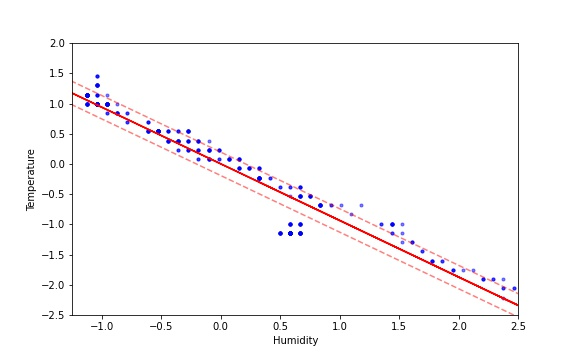
\includegraphics[scale=0.45]{SVR_representation.jpg}
\end{center}
\caption{\label{fig-SVRex}Visual Representation of an SVR}
\end{figure}

A multi-objective function is constructed from the loss function and the geometrical properties of the tube:

\begin{equation}\label{eqn:11}
    \min_{w, \xi, \hat{\xi} \in \mathbb{R}}{\frac{\parallel{w}\parallel^2}{2} + C\sum_{i=1}^n (\xi_i + \hat{\xi_i})}
\end{equation}
\begin{center}
subject to $\xi, \hat{\xi} \geq 0$, i=1,...,n \\ 
$w^T \cdot \Phi(x_i) + b - y_i \leq \epsilon + \xi_i$\\ 
$y_i - w^T \cdot \Phi(x_i) - b \leq  \epsilon + \hat{\xi_i} $ \\
\end{center}
where $\Phi(.)$ is the transformation to a kernel space and C is a regularization parameter which controls the strength of the penalty. C acts as an inverse regularization parameter since when it is large, more emphasis is placed on the error and when the opposite is true, more emphasis is placed on the norm of the weights. The values of $\xi$ and $\hat{\xi}$ follow a similar pattern as Equation \ref{eqn:10} where their values are zero if $y_i$ is inside the tube, otherwise $\xi$ is the positive difference between $y_i$ and $\epsilon$ and $\hat{\xi}$ will be nonzero if $y_i$ is below the tube. 

The corresponding Langrarian ($L_2=L(w,\xi,\hat{\xi},\lambda,\hat{\lambda},\alpha,\hat{\alpha})$) of Equation \ref{eqn:11}:

\begin{equation}\label{eqn:12}
\begin{aligned}
        L_2 = &  {\frac{\parallel{w}\parallel^2}{2} + C\sum_{i=1}^n (\xi_i + \hat{\xi_i})} - \\
        & {\sum_{i=1}^N\hat{\alpha_i}(y_i- w^T \cdot \Phi(x_i) -b + \epsilon + \hat{\xi_i})} - \\
        & {\sum_{i=1}^N\alpha_i(w^T \cdot \Phi(x_i) + b - y_i + \epsilon + \xi_i)} - \\
        & \sum_{i=1}^N(\lambda_i\xi_i+ \hat{\lambda_i}\hat{\xi_i})
\end{aligned}
\end{equation}
where $\lambda,\hat{\lambda},\alpha,\hat{\alpha}$ are the Lagrange multipliers and are all non-negative real numbers. The minimum of Equation \ref{eqn:12} can be found by differentiating with respect to the parameters ($w, b, \xi$) which results in the equivalent maximization of the following dual objective function:

\begin{equation}
\begin{aligned}
    \max_{\alpha,\hat{\alpha}}{y^T (\hat{\alpha} -\alpha) - \epsilon e^T(\hat{\alpha} +\alpha)  - \frac{1}{2}{(\alpha+\hat{\alpha})^TQ(\alpha-\hat{\alpha})}}
\end{aligned}
\end{equation}
\begin{center}
    subject to $e^T(\alpha-\hat{\alpha})=0$, $0 \leq \alpha_i,\hat{\alpha_i} \leq C, i=1,...,n$
\end{center}
where $e$ is a vector of all ones and $Q$ is the kernel matrix ($Q_{ij}=k(x_i,x_j) = (\Phi(x_i)^T \cdot \Phi(x_i))$. Assuming we have a new input $x_p$ we can use the following function to get its prediction value $y_p$:

\begin{equation}
    y_p = \sum_{i=1}^{N_{SV}}(\alpha_i-\hat{\alpha})k(x_i,x_p) + b
\end{equation}
where $N_{SV}$ denotes the number of support vectors and $k(x_i,$ $x_p)$ the kernel. In our experiments, we've set the SVR kernel to either be a linear or an RBF kernel (Equations \ref{eqn:linear} and \ref{eqn:rbf} respectively).

\section{Related Work}

Compute reuse has been investigated in the context of edge computing by \cite{ComputeReuse} to quantify its gain. Executing experiments on three applications: matrix multiplication, face detection, and chess, they found that systems that adopt compute reuse, compared to systems that don't, can finish the same task up to five times faster. In addition to the benefits of compute reuse they also highlight some challenges including task representation and privacy considerations. Model tasks need to have a clear specification detailing their purpose and speciality in order to identify when they can be re-used while also preserving user privacy when they are shared. Motivated by similar concerns a theoretical paradigm named learnware was proposed by Zhou \cite{Learnware}. More specifically, a learnware is a machine learning model that is pretrained and achieves good performance paired with a detailed specification. The vision behind the paradigm was that learnware models can be shared in a pool without their raw data, allowing data scientists to identify pretrained models that satisfy their requirements without concerns over privacy violations. Therefore, the author identified three characteristics: reusable, evolvable and comprehensible as fundamental for a model to be considered a learnware.  

Based on this paradigm, the reduced kernel mean embedding (RKME) \cite{KernelMMD} was presented, a two phased framework consisting of the upload and deployment phase. During the upload phase, each model is paired with its kernel mean embedding (KME) of the dataset and added to the pool of models. Roughly speaking, a kernel mean embedding is a point in the reproducing Hilbert space (RKHS) which "summarises" the probability distribution. Then in the deployment phase either a single or a combination of models is chosen based on the RKHS distance between the testing (target) mean embedding and reduced (source) embedding of pool models. Therefore, there is no need to access the raw data since KME acts a proxy for them. The RKME method is similar to the MMD  statistic \cite{OriginalMMD}, which is the largest difference between the mean embedding of two populations (source and target) and its aim is to determine if the two populations were drawn from the same distribution. Essentially, this is what the deployment phase of the framework does, it wants to find the model which minimises the difference and thus ensures that the target distribution is the same as the source. The framework was tested in a series of experiments including a real-world project where it outperformed reuse baselines in terms of the root-mean-square error.

The author of the learnware paradigm \cite{Learnware} recognises transfer learning as a preliminary attempt to reusability. The aim of transfer learning is to transfer the knowledge of a pretrained model to a new model that is used for a different but related problem. In transfer learning there are three key research issues as identified in \cite{DefinitionTL}: when, how and what to transfer. This corresponds to identifying a source domain that would benefit the target domain, then using an algorithm the transferable knowledge across domains is discovered. A two-stage framework dubbed as Learning to Transfer (L2T) was presented \cite{L2T}, which exploits previous transfer learning experiences to optimize what and how to transfer between domains. In the first stage each transfer learning experience is encoded into three parts: a pair of source and target domains, the transferred knowledge between them represented by latent factors and the performance improvement ratio. Using these transfer learning experiences, L2T learns a reflection function, which approximates the performance improvement ratio and thus encrypts transfer learning skills of deciding what and how to transfer. The improvement ratio in this framework is the difference between domains calculated by MMD further highlighting the similarity to RKME \cite{KernelMMD}. In addition to the MMD between domains, the variance is also calculated since a small MMD paired with an extremely high variance still indicates little overlap. A potential drawback of the RKME \cite{KernelMMD} framework, and by extension the learnware paradigm, is that the variance between pairs cannot be calculated since the raw data are not available during the testing phase. During the second stage, whenever a new pair of domains arrives, L2T optimizes the knowledge to be transferred by maximising the value of the learned reflection function.

Concerns over intellectual property (IP) infringement and vulnerability propagation of deep learning models (DNN) motivated the proposal of ModelDiff \cite{DNNSimilarity}, a testing-based approach to DNN model similarity comparison. They compare the decision logic of models on the test inputs represented by a decision distance vector (DDV),a newly defined data structure in which each value is the distance between the outputs of the model produced by two inputs. These inputs are pairs of normal and corresponding adversarial samples and thus when used to calculate the DDV, the decision boundary is captured. In contrast to RKME \cite{KernelMMD} which is a compute reuse framework, ModelDiff is a model reuse detector. 

Model reuse has also been used to handle concept drift, a situation where the distribution of the data (usually stream data) changes. The assumption that previous data contain some useful information, indicates that the models corresponding to the data can be leveraged. Condor was proposed \cite{ConceptDrift} as an approach to handling concept drift through model reuse. Condor consists of two modules, ModelUpdate and WeightUpdate which leverage previous knowledge to build new model, hence updating the model pool and adapt the weights of previous models to reflect current reusability performance respectively. The effectiveness of the approach was validated using both synthetic and real-world datasets. 

Hasani et al. \cite{MaterializationReuse} proposed a two-phased approach, to build faster models for a popular class of analytic queries by leveraging model reuse. Similar to other approaches such as RKME \cite{KernelMMD}, there is a preprocessing and a runtime phase. During the first phase the models, their statistics and some meta-data are stored, while in the second phase relevant models are identified from which an approximate model is constructed. Moreover, they propose two methods for generating approximate models, one which is extremely fast but does not provide a fine-tuning option and another which does at the cost of efficiency. Their approach can achieve speed-ups of several orders on magnitude on very large datasets, however it is only geared towards exploratory analysis purposes and the approach is potentially less robust under concept drift. 

Lee et al. \cite{ComputeReuse} also discuss alternative approaches and corresponding challenges of compute reuse including in networks. They identify that reuse can be achieved either in a distributed or centralized manner. The distributed approach involves forwarding tasks to the compute reuse node that is responsible for the operation. This adds additional complexity to the forwarding operations of routers resulting in a potential downgrade in performance. Reuse of results in a network setting undoubtedly improves performance, however speeding up the estimation of parameters can also be beneficial in that regard. Nodes in a network can collaborate to estimate parameters as discussed in \cite{DistributedEstimation}. More specifically, their method takes advantage of the joint sparsity of vectors used for computations enhancing estimation performance. Joint sparsity simply means that the indexes of nonzero entries for all nodes are the same, but their values differ.  The authors also adopt an intertask cooperation strategy to consider intertask similarities. Their method assumes that both the vectors of interest and their associated noise follow a zero-mean Gaussian distribution which is a strong assumption for the data to hold. 

In conclusion, reusing models results in significant reduction in compute usage resources. Both theoretical and empirical frameworks have been proposed to take advantage of the performance improvement of model reusability. Nevertheless, model reuse has also been used to tackle concept drift and building ad-hoc analytic models. While model reuse is undoubtedly beneficial many have raised concerns including user privacy and intellectual property considerations.  These are legitimate concerns of model sharing, however  our model reuse  framework is novel and therefore user privacy is not a concern at this stage of development. In the future we could amend the framework to not expose any data outside of the node. At this stage we've investigated whether the framework is feasible. In contrast to previous research in which frameworks required two distinct steps, our framework is online, and they are therefore merged. Our framework includes determining which datasets are similar, but also the direction of reusability.  Similarly, to the L2T \cite{L2T} framework we use MMD to measure the similarity of two dataset domains. In previous research there was no requirement to determine the direction of reusability hence we propose a novel approach, using the OCSVM model of each node to predict other node’s inliers and measuring the overlap.

% \begin{table}
% \begin{tabular}{l||c||p{2cm}}
% % \emph{Operating System} & \emph{Version} & \emph{Verdict} \\ \hline \hline
% % Ubuntu & 12.04 & Everyone's favourite Linux, unless you grew up with
% % RedHat \\ \hline
% % Slackware & xxx & Pseudo-hacker's Linux, how often do you recompile
% % your kernel? \\ \hline
% % Mac OS & 10.7 & For people with more money than sense \\ \hline
% \end{tabular}
% \caption{\label{tab-eg}Single column table of figures}
% \end{table}

% \begin{lstlisting}[language=python,caption={The algorithm for OCSVM model 1}, label=lst:ocsvm1]
% def avg_similarity_disimilarity_MMD(samples, similar_nodes, other_nodes, 
%                                     kernel, kernel_bandwidth, return_tables = True):
    
%     ## Calculating the baseline ASMMD
%     combos = comb(range(len(similar_nodes)),2)
%     similar_mmds = []
%     for combo in combos:
%         x = similar_nodes[combo[0]]
%         y = similar_nodes[combo[1]]
%         sx = samples[x]
%         sy = samples[y]
%         mmd = MMD(sx,sy, kernel, kernel_bandwidth)
%         similar_mmds.append(mmd)
%         s.add_row([(x,y), mmd])

% \end{lstlisting}

\section{The Similar Pairs Algorithms}

In our experiments we've utilised two methods to determine pair similarity, one based on MMD and the other on OCSVM. In both cases we need to examine every pair combination and determine which of those pairs are similar based on a threshold. 

% NOTE: line ends are denoted by \; in algorithm2e

\SetInd{0.1em}{0.75em}
\SetNlSkip{0.5em}

\begin{algorithm}
    \DontPrintSemicolon
    \caption{Calculates the average similarity MMD (ASMMD) between the given nodes.
    }\label{alg:asmmd}
    
    \KwData{$\boldsymbol{samples}$: dictionary associating each node (pi2-pi5) with a sample used for the MMD calculation, $\boldsymbol{similar\_nodes}$: nodes which we have visually identified as similar to each other, $\boldsymbol{other\_nodes}$: the rest of the nodes, $\boldsymbol{kernel}, \boldsymbol{bandwidth}$: the kernel type and scalar value to be used for the MMD calculation.}
    \KwResult{ASMMD}

    \Begin{ 
        \tcp{Calculating the baseline ASMMD}
        $similar\_mmds \longleftarrow \left[\right]$ \;
        \SetAlgoLined
        \SetKw{KwTo}{in}
        \For{$x, y$ \KwTo $get\_pair\_combos(similar\_nodes)$}{
            $sx \longleftarrow samples[x]$, $sy \longleftarrow samples[y]$ \;
            $mmd \longleftarrow MMD(sx, sy, kernel, bandwidth)$ \;
            $similar\_mmds.append(mmd)$ \;
        }
        \tcp{Compare whether any of the other\_nodes are similar to any of the similar\_nodes using the baseline ASMMD}
        \For{$x$ \KwTo $other\_nodes$}{
            $sx \longleftarrow samples[x]$ \;
            \For{$y$ \KwTo $similar\_nodes$}{
                $sy \longleftarrow samples[y]$ \;
                $mmd \longleftarrow MMD(sx, sy, kernel, bandwidth)$ \;
                $current\_asmmd \longleftarrow \boldsymbol{mean}(similar\_mmds)$ \;
                \If{$mmd < (current\_asmmd + 1) * 0.05$}{
                    $similar\_mmds.append(mmd)$}
            }
        }
        \tcp{Compare whether any of the other\_nodes are similar to each other using the current ASMMD}
        \If{$\boldsymbol{len}(other\_nodes>1)$}{
            \For{$x, y$ \KwTo $get\_pair\_combos(other\_nodes)$}{
                $sx \longleftarrow samples[x]$, $sy \longleftarrow samples[y]$ \;
                $mmd \longleftarrow MMD(sx, sy, kernel, bandwidth)$ \;
                $current\_asmmd \longleftarrow \boldsymbol{mean}(similar\_mmds)$ \;
                \If{$mmd < (current\_asmmd + 1) * 0.05$}{
                    $similar\_mmds.append(mmd)$}
            }
        }
        $asmmd = \boldsymbol{mean}(similar\_mmds)$ \;
    }
\end{algorithm}

For the MMD method this threshold is called the average similarity MMD (ASMMD), a value calculated using Algorithm \ref{alg:asmmd}. Algorithm \ref{alg:asmmd} requires that we categorise nodes into two sets, one where all nodes are similar to each other and the rest of them. We calculate a baseline ASMMD by calculating the MMD of all pair combinations of the similar nodes. Then, we use ASMMD (allowing for a 5\% variation) to judge whether the rest of the nodes are similar to each other or to the similar nodes. If they are we calculate the new ASMMD and we use this to judge the next pair. Using the result of this process we can then judge which pairs are similar for a given experiment as demonstrated in Algorithm  \ref{alg:mmd_pairs}. 

\begin{algorithm}
    \DontPrintSemicolon
    \caption{Finds the MMD based similar pairs
    }\label{alg:mmd_pairs}
    
    \KwData{$\boldsymbol{samples}$: dictionary associating each node (pi2-pi5) with a sample, $\boldsymbol{asmmd}$: average similarity (ASMMD) calculated using Algorithm \ref{alg:asmmd}, $\boldsymbol{kernel}, \boldsymbol{bandwidth}$: the kernel type and scalar value to be used for the MMD calculation.}
    \KwResult{$similar\_pairs, pair\_mmds$}
    
    \Begin{
        $similar\_pairs \longleftarrow []$ \;
        % $similar\_nodes \longleftarrow []$ \;
        $pair\_mmds \longleftarrow []$\;
        $nodes \longleftarrow ["pi2", "pi3", "pi4", "pi5"]$ \; 
        \SetAlgoLined
        \SetKw{KwTo}{in}
        \For{x, y \KwTo $get\_pair\_combos(nodes)$}{
            $sx \longleftarrow samples[x]$, $sy \longleftarrow samples[y]$ \;
            $mmd \longleftarrow MMD(sx, sy, kernel, bandwidth)$ \;
            \If {$mmd < (asmmd + 1) * 0.05$}{
                % \If{x $\boldsymbol{not\ in}$ similar\_nodes}{
                %     $similar\_nodes.append(x)$
                % }
                % \If{y $\boldsymbol{not\ in}$ similar\_nodes}{
                %     $similar\_nodes.append(y)$
                % }
                $similar\_pairs.append((x,y))$ \;
                $pair\_mmds.append((mmd,mmd))$ \;
            }
        }
    }
\end{algorithm}

In the OCSVM method on the other hand this threshold is set by the user. Assuming we have two nodes $x$ and $y$, the threshold represents the minimum probability that the OCSVM model of node $x$, can correctly predict that the points of node $y$ are inliers and vice versa. In Algorithm \ref{alg:ocsvm_pairs} we calculate the probabilities in both directions and if at least one of them is higher than the threshold we deem that the pair of nodes is similar. 

\begin{algorithm}
    \DontPrintSemicolon
    \caption{Finds the OCSVM based similar pairs
    }\label{alg:ocsvm_pairs}
    
    \KwData{$\boldsymbol{samples}$: dictionary associating each node (pi2-pi5) with a sample, $\boldsymbol{models}$: dictionary associating each node with its OCSVM node model, $\boldsymbol{threshold}$: the minimum probability value for nodes to be considered similar}
    \KwResult{$similar\_pairs, pair\_prob$}
    
    \Begin{
        $similar\_pairs \longleftarrow []$ \;
        % $similar\_nodes \longleftarrow []$ \;
        $pair\_prob \longleftarrow []$\;
        $nodes \longleftarrow ["pi2", "pi3", "pi4", "pi5"]$ \;  \SetAlgoLined
        \SetKw{KwTo}{in}
        \For{x, y \KwTo $get\_pair\_combos(nodes)$}{
            $sx \longleftarrow samples[x]$, $sy \longleftarrow samples[y]$ \;
            $pred\_y\_inliers \longleftarrow get\_inliers(models[x], sy)$, 
            $pred\_x\_inliers \longleftarrow get\_inliers(models[y], sx)$  \;
            $x\_y\_overlap \longleftarrow \boldsymbol{len}(pred\_y\_inliers)/\boldsymbol{len}(sy)$,
            $y\_x\_overlap \longleftarrow \boldsymbol{len}(pred\_x\_inliers)/\boldsymbol{len}(sx)$ \;
            \If{$\boldsymbol{max}$(x\_y\_overlap, y\_x\_overlap) > threshold}{
                % \If{x $\boldsymbol{not\ in}$ similar\_nodes}{
                %     $similar\_nodes.append(x)$
                % }
                % \If{y $\boldsymbol{not\ in}$ similar\_nodes}{
                %     $similar\_nodes.append(y)$
                % }
                $similar\_pairs.append((x,y))$ \;
                $pair\_prob.append((x\_y\_overlap,y\_x\_overlap))$ \;
            }
        }
    }
\end{algorithm}

The idea behind the OCSVM-based method is that if the OCSVM model of node $x$ yields a high probability of correctly predicting inliers for node $y$, then potentially the model of node $x$ can be reused as a model for node $y$. Therefore, since we can have separate values per direction (forward (x,y), backward (y,x)) determining the degree of similarity between the two nodes we can also determine the direction of reusability. This an advantage of the OCSVM method compared to the MMD one as it can not only point towards the pairs that are similar but it can also determine which node model to reuse. 



% \subsection{User Interface}

% Blah blah blah
% Blah blah blah
% Blah blah blah
% Blah blah blah

% % - - - - - - - - - - - - - - - - - - - - - - - - - - - - - - - - - - - - - - -
% \subsection{Foo}

% Blah blah blah
% Blah blah blah
% Blah blah blah

% \subsubsection{Bar}
% \textsf{Blah} \textit{blah} \textbf{blah}

\section{Evaluation}

\subsection{Training Data}

For the purposes of our model we've experimented with the \textbf{\textit{GNFUV Unmanned Surface Vehicles Sensor Data Set}} \cite{Dataset} which includes data from three experiments. In each experiment there are four sets of mobile sensor readings data recorded by the Raspberry Pi's corresponding to four Unmanned Surface Vehicles (USVs). Each node (USV) dataset contains the humidity and temperature recorded when they were floating over the sea surface in a GPS pre-defined trajectory in a coastal area of Athens (Greece). The data description can be found in Table \ref{tab:Data Description}.

\begin{table*}[]
\centering
\begin{tabular}{|cccccccccc|}
\hline
\multicolumn{10}{|c|}{\textbf{Experiment 1}}                                                                                                                                   \\ \hline
\multicolumn{1}{|c|}{\textbf{Node}} & \multicolumn{1}{c|}{\textbf{No. of Entries}} & \multicolumn{4}{c|}{\textbf{Humidity}}        & \multicolumn{4}{c|}{\textbf{Temperature}} \\ \hline
\multicolumn{1}{|c|}{\textbf{}}     & \multicolumn{1}{c|}{\textbf{}}               & Min & Max & Avg   & \multicolumn{1}{c|}{Std}  & Min     & Max     & Avg       & Std       \\
\multicolumn{1}{|c|}{pi2}           & \multicolumn{1}{c|}{1532}                    & 3   & 45  & 35.85 & \multicolumn{1}{c|}{6.57} & 15      & 57      & 27.6      & 11.08     \\
\multicolumn{1}{|c|}{pi3}           & \multicolumn{1}{c|}{899}                     & 19  & 33  & 28.53 & \multicolumn{1}{c|}{4.39} & 34      & 59      & 43.04     & 6.17      \\
\multicolumn{1}{|c|}{pi4}           & \multicolumn{1}{c|}{1766}                    & 18  & 45  & 35.47 & \multicolumn{1}{c|}{6.55} & 0       & 64      & 28.2      & 11.71     \\
\multicolumn{1}{|c|}{pi5}           & \multicolumn{1}{c|}{2078}                    & 18  & 37  & 27.51 & \multicolumn{1}{c|}{5.1}  & 20      & 63      & 39.78     & 6.9       \\ \hline
\multicolumn{10}{|c|}{\textbf{Experiment 2}}                                                                                                                                   \\ \hline
\multicolumn{1}{|c|}{pi2}           & \multicolumn{1}{c|}{580}                     & 26  & 56  & 48.48 & \multicolumn{1}{c|}{6.6}  & 21      & 49      & 28.42     & 3.86      \\
\multicolumn{1}{|c|}{pi3}           & \multicolumn{1}{c|}{807}                     & 27  & 49  & 41.73 & \multicolumn{1}{c|}{4.14} & 17      & 46      & 23.41     & 5.66      \\
\multicolumn{1}{|c|}{pi4}           & \multicolumn{1}{c|}{1021}                    & 30  & 59  & 50.56 & \multicolumn{1}{c|}{6.4}  & 16      & 36      & 22.76     & 2.76      \\
\multicolumn{1}{|c|}{pi5}           & \multicolumn{1}{c|}{1407}                    & 30  & 48  & 40.13 & \multicolumn{1}{c|}{2.73} & 20      & 49      & 28.05     & 3.36      \\ \hline
\multicolumn{10}{|c|}{\textbf{Experiment 3}}                                                                                                                                   \\ \hline
\multicolumn{1}{|c|}{pi2}           & \multicolumn{1}{c|}{342}                     & 33  & 42  & 38.39 & \multicolumn{1}{c|}{2.39} & 17      & 31      & 23.44     & 4.09      \\
\multicolumn{1}{|c|}{pi3}           & \multicolumn{1}{c|}{264}                     & 27  & 33  & 31.95 & \multicolumn{1}{c|}{0.77} & 34      & 43      & 38.63     & 1.26      \\
\multicolumn{1}{|c|}{pi4}           & \multicolumn{1}{c|}{488}                     & 20  & 39  & 31.24 & \multicolumn{1}{c|}{5.31} & 23      & 59      & 38.28     & 10.56     \\
\multicolumn{1}{|c|}{pi5}           & \multicolumn{1}{c|}{555}                     & 21  & 37  & 25.23 & \multicolumn{1}{c|}{3.91} & 20      & 47      & 38.13     & 4.65      \\ \hline
\end{tabular}
\caption{\label{tab:Data Description}Dataset Description}
\end{table*}

% Graphs are always good. I recommend getting to grips with Matlab, R or
% gnuplot rather than exporting horribly Excel bitmapped graphs.


% \begin{quotation}
%  The Assyrian came down like the wolf on the fold,
%  And his cohorts were gleaming in purple and gold;
%  And the sheen of their spears was like stars on the sea,
%  When the blue wave rolls nightly on deep Galilee.

%  Like the leaves of the forest when Summer is green,
%  That host with their banners at sunset were seen:
%  Like the leaves of the forest when Autumn hath blown,
%  That host on the morrow lay withered and strown.
% \end{quotation}

\section{Conclusions}

% The standard Lorem Ipsum passage, used since the 1500s

% ``Lorem ipsum dolor sit amet, consectetur adipisicing elit, sed do eiusmod tempor incididunt ut labore et dolore magna aliqua. Ut enim ad minim veniam, quis nostrud exercitation ullamco laboris nisi ut aliquip ex ea commodo consequat. Duis aute irure dolor in reprehenderit in voluptate velit esse cillum dolore eu fugiat nulla pariatur. Excepteur sint occaecat cupidatat non proident, sunt in culpa qui officia deserunt mollit anim id est laborum.''
\vskip8pt \noindent
{\bf Acknowledgments.}
This is optional; it is a location for you to thank people

\bibliographystyle{acm}
\bibliography{thesis}


\end{document}